\documentclass{article}

\usepackage{amsmath,amsfonts,amsthm,amssymb,amsopn,bm,mathtools}

\usepackage[margin=.9in]{geometry}
\usepackage{graphicx}
\usepackage{url}
\usepackage[hidelinks]{hyperref}
\usepackage[usenames,dvipsnames]{color}
\usepackage{fancyhdr}
\usepackage{multirow}
\usepackage{mdframed}
\usepackage{ifthen}
\usepackage[shortlabels]{enumitem}
\usepackage{fancyhdr}
\usepackage{hyperref}
\usepackage{mathtools}
\usepackage{ifthen}
\usepackage[ruled]{algorithm2e}

\newcommand{\field}[1]{\mathbb{#1}}
\newcommand{\1}{\mathbf{1}}
% \newcommand{\E}{\mathbb{E}}
\renewcommand{\P}{\mathbb{P}}
\newcommand{\R}{\field{R}} % real domain
% \newcommand{\C}{\field{C}} % complex domain
\newcommand{\F}{\field{F}} % functional domain

\newcommand{\T}{^{\textrm T}} % transpose
\newcommand{\bx}{\mathbf x}
\newcommand{\by}{\mathbf y}
\newcommand{\bw}{\mathbf w}

\providecommand*{\eu}{\ensuremath{\mathrm{e}}}
\def\diag{\text{diag}}


%% operator in linear algebra, functional analysis
\newcommand{\inner}[2]{#1\cdot #2}
% \newcommand{\norm}[1]{\left\| #1 \right\|}
% \newcommand{\twonorm}[1]{\|#1\|_2^2}
% operator in functios, maps such as M: domain1 --> domain 2
\newcommand{\Map}[1]{\mathcal{#1}}
\renewcommand{\theenumi}{\alph{enumi}} 

\newcommand{\Perp}{\perp \! \! \! \perp}

\newcommand\independent{\protect\mathpalette{\protect\independenT}{\perp}}
\def\independenT#1#2{\mathrel{\rlap{$#1#2$}\mkern2mu{#1#2}}}
\newcommand{\vect}[1]{\mathbf{#1}} % vector
\newcommand{\mat}[1]{\mathbf{#1}} % matrix
\newcommand{\cst}[1]{\mathsf{#1}} % constant
\newcommand{\ProbOpr}[1]{\mathbb{#1}}
\newcommand{\points}[1]{\small\textcolor{magenta}{\emph{[#1 point\ifthenelse{\equal{#1}{1}}{}{s}]}} \normalsize}

\newcounter{aprob}
\newenvironment{aprob}[1][]{\refstepcounter{aprob}\par\medskip\noindent A\theaprob.#1 }

 \newcounter{bprob}
\newenvironment{bprob}[1][]{\begin{mdframed} \refstepcounter{bprob}\par\medskip
  B\thebprob.#1 }
   { \end{mdframed} }

\usepackage{amsmath,amsfonts,amsthm,amssymb,amsopn,bm,mathtools}
\usepackage[margin=.9in]{geometry}
\usepackage{graphicx}
\usepackage{url}
\usepackage[hidelinks]{hyperref}
\usepackage[usenames,dvipsnames]{color}
\usepackage{fancyhdr}
\usepackage{multirow}
\usepackage{mdframed}
\usepackage{ifthen}

% calculus
% the differential operator
\makeatletter
\providecommand*{\diff}
{\@ifnextchar^{\DIfF}{\DIfF^{}}}
\def\DIfF^#1{
	\mathop{\mathrm{\mathstrut d}}
	\nolimits^{#1}\gobblespace}
\def\gobblespace{
	\futurelet\diffarg\opspace}
\def\opspace{
	\let\DiffSpace\!
	\ifx\diffarg(
	\let\DiffSpace\relax
	\else
	\ifx\diffarg[
	\let\DiffSpace\relax
	\else
	\ifx\diffarg\{
	\let\DiffSpace\relax
	\fi\fi\fi\DiffSpace}

\providecommand*{\pdiff}
{\@ifnextchar^{\pDIfF}{\pDIfF^{}}}
\def\pDIfF^#1{
	\mathop{\mathrm{\mathstrut \partial}}
	\nolimits^{#1}\gobblespace}
\def\gobblespace{
	\futurelet\diffarg\opspace}
\def\opspace{
	\let\DiffSpace\!
	\ifx\diffarg(
	\let\DiffSpace\relax
	\else
	\ifx\diffarg[
	\let\DiffSpace\relax
	\else
	\ifx\diffarg\{
	\let\DiffSpace\relax
	\fi\fi\fi\DiffSpace}

% derivative and partial derivative operators
\providecommand*{\deriv}[3][]{\frac{\diff^{#1}{#2}}{\diff {#3}^{#1}}}
\providecommand*{\pderiv}[3][]{\frac{\pdiff^{#1}{#2}}{\pdiff {#3}^{#1}}}
\providecommand*{\pderivcross}[3]{\frac{\pdiff^{2} {#1}}{\pdiff {#2} \pdiff {#3} }}

% set notation
\providecommand\given{}
\newcommand\SetSymbol[1][]{%
	\nonscript\:#1\vert
	\allowbreak
	\nonscript\:
	\mathopen{}}
\DeclarePairedDelimiterX\Set[1]\{\}{%
	\renewcommand\given{\SetSymbol[\delimsize]}
	#1
}
\newcommand{\set}[1]{\Set*{#1}}


% probability
\DeclarePairedDelimiterXPP\prob[1]{\mathop{\mathbb{P}}}{\lbrace}{\rbrace}{}{\renewcommand\given{\nonscript\:\delimsize\vert\nonscript\:\mathopen{}}#1}
\newcommand{\Prob}[1]{\prob*{#1}}

\DeclarePairedDelimiterXPP\probability[2]{\mathop{\mathbb{P}}_{#1}}{\lbrace}{\rbrace}{}{\renewcommand\given{\nonscript\:\delimsize\vert\nonscript\:\mathopen{}}#2}
\newcommand{\Probability}[2]{\probability*{#1}{#2}}

\DeclarePairedDelimiterXPP\expectation[1]{\mathop{\mathbb{E}}}{\lbrack}{\rbrack}{}{\renewcommand\given{\nonscript\:\delimsize\vert\nonscript\:\mathopen{}}#1}
\newcommand{\E}[1]{\expectation*{#1}}

\DeclarePairedDelimiterXPP\expectationdist[2]{\mathop{\mathbb{E}}_{#1}}{\lbrack}{\rbrack}{}{\renewcommand\given{\nonscript\:\delimsize\vert\nonscript\:\mathopen{}}#2}
\newcommand{\Exp}[2]{\expectationdist*{#1}{#2}}

\DeclarePairedDelimiterXPP\variance[1]{\mathop{\mathrm{Var}}}{\lbrack}{\rbrack}{}{\renewcommand\given{\nonscript\:\delimsize\vert\nonscript\:\mathopen{}}#1}
\newcommand{\Var}[1]{\variance*{#1}}

\DeclarePairedDelimiterXPP\variancedist[2]{\mathop{\mathrm{Var}}_{#1}}{\lbrack}{\rbrack}{}{\renewcommand\given{\nonscript\:\delimsize\vert\nonscript\:\mathopen{}}#2}
\newcommand{\Variance}[2]{\variancedist*{#1}{#2}}

\DeclarePairedDelimiterXPP\covariance[2]{\mathop{\mathrm{Cov}}}{(}{)}{}{#1,\mathopen{}#2}
\newcommand{\Cov}[2]{\covariance*{#1}{#2}}


% Linear Algebra, symmetry notation
\newcommand{\Matrix}[1]{\begin{bmatrix}#1\end{bmatrix}}
\newcommand{\Tr}[1]{\mathop{\mathrm{Tr}}\squarebrack{#1}}

% norms
\DeclarePairedDelimiterXPP{\nrm}[2]{}{\lVert}{\rVert}{\ensuremath{_{#1}}}{\ifblank{#2}{\:\cdot\:}{#2}}
\newcommand{\norm}[2]{\nrm*{#1}{#2}}

\newcommand{\twonorm}[1]{\norm{2}{#1}}
\newcommand{\twonormsq}[1]{\norm{2}{#1}^2}
\newcommand{\opnorm}[1]{\norm{\mathrm{op}}{#1}}
\newcommand{\normF}[1]{\norm{\mathrm{F}}{#1}}


% parentheses
\DeclarePairedDelimiterX{\bracket}[3]{#1}{#2}{#3}

\newcommand{\abs}[1]{\bracket*{\lvert}{\rvert}{#1}}
\newcommand{\round}[1]{\bracket*{(}{)}{#1}}
\newcommand{\curly}[1]{\bracket*{\lbrace}{\rbrace}{#1}}
\newcommand{\squarebrack}[1]{\bracket*{\lbrack}{\rbrack}{#1}}

% For Convenience
\newcommand{\comment}[1]{\qquad\round{\text{#1}}}
\newcommand{\commentnewline}[1]{\qquad\qquad\qquad\qquad\qquad\qquad\comment{#1}\nonumber}
\newcommand{\inv}[1]{\frac{1}{#1}}
\newcommand{\sumi}[2]{\sum\limits_{i=#1}^{#2}}
\newcommand{\sumj}[2]{\sum\limits_{j=#1}^{#2}}
\newcommand{\sumk}[2]{\sum\limits_{k=#1}^{#2}}

\newcommand{\field}[1]{\mathbb{#1}}
\newcommand{\1}{\mathbf{1}}
\newcommand{\R}{\field{R}} % real domain
\newcommand{\bx}{\mathbf{x}}

% TODO command
\usepackage{xcolor}
\newcommand{\todo}{\textcolor{red!90!black}{\textbf{TODO}}}

\def\diag{\text{diag}}

%% operator in linear algebra, functional analysis
\newcommand{\inner}[2]{#1\cdot #2}
\renewcommand{\theenumi}{\alph{enumi}} 

\newcommand{\Perp}{\perp \! \! \! \perp}

\newcommand\independent{\protect\mathpalette{\protect\independenT}{\perp}}
\def\independenT#1#2{\mathrel{\rlap{$#1#2$}\mkern2mu{#1#2}}}
\newcommand{\vct}[1]{\mathbf{#1}} % vector
\newcommand{\vect}[1]{\mathbf{#1}} % vector
\newcommand{\mat}[1]{\mathbf{#1}} % matrix
\newcommand{\cst}[1]{\mathsf{#1}} % constant
\newcommand{\points}[1]{\small\textcolor{magenta}{\emph{[#1 point\ifthenelse{\equal{#1}{1}}{}{s}]}} \normalsize}

% Define a new problem
\newcounter{aprob}
\newenvironment{aprob}[1][]{\refstepcounter{aprob}\par\medskip\noindent A\theaprob.#1 }

\newcounter{bprob}
\newenvironment{bprob}[1][]{\begin{mdframed} \refstepcounter{bprob}\par\medskip\noindent B\thebprob.#1 }
  {\vspace{1pt} \end{mdframed}}


\usepackage{listings}  % Include the listings-package
\lstset{language=Python}
\usepackage{float}
\usepackage{multicol}
\usepackage{enumitem}
\usepackage{wrapfig}

\def\P{\mathbb{P}}
\def\R{\mathbb{R}}

\newtheorem{lemma}{Lemma}

\DeclareMathOperator*{\argmax}{arg\,max} 
\DeclareMathOperator*{\argmin}{arg\,min} 
\global\long\def\dd{\textnormal{d}}


\date{{}}

\setlength\parindent{0px}

\begin{document}
\setcounter{aprob}{0}
\title{Homework \#3}
\author{
    \normalsize{CSE 446/546: Machine Learning}\\
    \normalsize{Profs. Jamie Morgenstern and Simon Du}\\
    \normalsize{Sami Turbeville; \textbf{Collab:} Shabab Ahmed }\\
    \normalsize{Due: \textbf{Wednesday} November 17, 2021 11:59pm}\\
    \normalsize{\textbf{A:} 71 points, \textbf{B:} 15 points}
}
\date{{}}
\maketitle

% \noindent Please review all homework guidance posted on the website before submitting to GradeScope. Reminders:
% \begin{itemize}
%     \item Make sure to read the ``What to Submit'' section following each question and include all items.
%     \item Please provide succinct answers and supporting reasoning for each question. Similarly, when discussing experimental results, concisely create tables and/or figures when appropriate to organize the experimental results. All explanations, tables, and figures for any particular part of a question must be grouped together. 
%     \item For every problem involving generating plots, please include the plots as part of your PDF submission.
%     \item When submitting to Gradescope, please link each question from the homework in Gradescope to the location of its answer in your homework PDF. Failure to do so may result in deductions of up to \points{5}. For instructions, see \url{https://www.gradescope.com/get_started#student-submission}.
%     \item Please recall that B problems, indicated in \boxed{\textrm{boxed text}}, are only graded for 546 students, and that they will be weighted at most 0.2 of your final GPA (see the course website for details). In Gradescope, there is a place to submit solutions to A and B problems separately. You are welcome to create a single PDF that contains answers to both and submit the same PDF twice, but associate the answers with the individual questions in Gradescope. 
%     \item If you collaborate on this homework with others, you must indicate who you worked with on your homework. Failure to do so may result in accusations of plagiarism.
%     \item For every problem involving code, please submit your code to the separate assignment on Gradescope created for code. Not submitting all code files will lead to a deduction of \points{1}.  
%     \item Please indicate your final answer to each question by placing a box around the main result(s). To do this in \LaTeX, one option is using the \texttt{boxed} command.
% \end{itemize}

% Not adhering to these reminders may result in point deductions. \\

% \textcolor{red}{\textbf{Changelog:}}

% \begin{itemize}
%     \item \textbf{Date:} Changed This.
% \end{itemize}

% \clearpage{}

\section*{Short Answer and ``True or False'' Conceptual Questions}
\begin{aprob}
    The answers to these questions should be answerable without referring to external materials. Briefly justify your answers with a few words.
    \begin{enumerate}
        \item \points{2} Say you trained an SVM classifier with an RBF kernel 
        ($K(u, v) = \exp\left(- \frac{{\| u-v \| }^2_2}{2\sigma^2} \right)$). 
        It seems to underfit the training set: should you increase or decrease $\sigma$?
        
        \textbf{Solution}: Decrease the bandwidth $\sigma$ to get a better fit because you are decreasing the bias. Bias-variance trade off means you need to be careful how much to decrease the bias before we start overfitting.

        \newpage
        \item \points{2} True or False:   Training deep neural networks requires minimizing a non-convex loss function, and therefore gradient descent might not reach the globally-optimal solution.
        
        \textbf{Solution:} True, the gradient can either blow up or go to zero, so we use SGD, but we could use for something else too.
        
        \newpage
        \item \points{2} True or False: It is a good practice to initialize all weights to zero when training a deep neural network.
        
        \textbf{Solution}: False, we initialize the weights with a random generator.

        \newpage
        \item \points{2} True or False: We use non-linear activation functions in a neural network’s hidden layers so that the network learns non-linear decision boundaries.
        
        \textbf{Solution:} True, we use non-linear activtion in between linear hidden layers to improve the model's accuracy by learning non-linear boundaries as well.
        
        \newpage
        \item \points{2} True or False: Given a neural network, the time complexity of the backward pass step in the backpropagation algorithm can be prohibitively larger compared to the relatively low time complexity of the forward pass step.
        
        \textbf{Solution:} False. the complexity of backwards and forward pass is the same up to a constant.

        \newpage
        \item \points{2} True or False: Neural Networks are the most extensible model and therefore the best choice for every circumstance.
        
        \textbf{Solution:} False, never say never. While NN are very extensible and a good choice for most circumstances, there are some circumstanes in which another type of Machine Learning may be better used - something like determining the price of a house given paramters such as \# of bedrooms, square footage, \# of bathrooms, etc. We want these paramters to be defined by us not some mystery parameter defined by the NN.

    \end{enumerate}
    % \subsection*{What to Submit:}
    % \begin{itemize}
    %     \item \textbf{Parts a-f:} 1-2 sentence explanation containing your answer.
    % \end{itemize}
\end{aprob}

\newpage

\section*{Support Vector Machines}
\begin{aprob}
    Assume $w$ is an $n$-dimensional vector and $b$ is a scalar. A hyperplane in $\R^n$ is the set $\set{x\in \R^n\given w^\top x + b = 0}$.
    \begin{enumerate}
    	\item \points{1} ($n=2$ example) Draw the hyperplane for $w=\Matrix{-1 & 2}^\top$, $b=2$? Label your axes.

        \textbf{Solution:} When $w=\Matrix{-1 & 2}^\top$ and $b=2$ then 
        \[ w^\top x + b = 0 \]
        \[ \Matrix{-1 & 2} \Matrix{x_1 \\ x_2} = -2 \]
        \[ -x_1 + 2 x_2 = -2 \]
        \[ x_2 = \frac{1}{2} x_1 - 1 \]
        Thus, the hyperplane looks like:
        \begin{figure}[h]
            \centering
            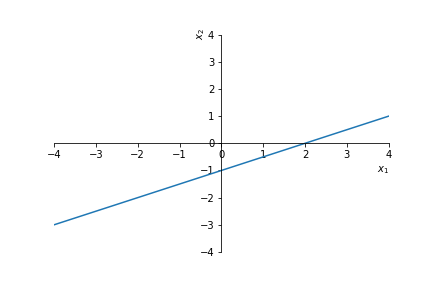
\includegraphics[width=0.6\textwidth]{a2a_hyperplane.png}
            \caption{hyperplane $x$ when $w = \Matrix{-1 \\ 2}$}\label{fig:a2a}
        \end{figure}

        \newpage

    	\item \points{1} ($n=3$ example) Draw the hyperplane for $w=\Matrix{1 & 1 & 1}^\top$, $b=0$? Label your axes.
    	
        \textbf{Solution:} When $w = \Matrix{1 \\ 1 \\1 }$ and $b=0$, then the hyperplane $x$ is:

        \[ x_1 + x_2 + x_3 = 0 \]

        \begin{figure}[h]
            \centering
            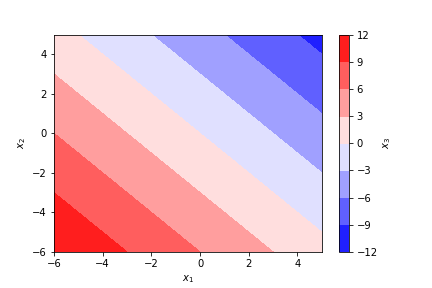
\includegraphics[width=0.6\textwidth]{a2b_hyperplane3d.png}
            \caption{hyperplane $x$ when $w = \Matrix{1 \\ 1 \\1}$}\label{fig:a2b}
        \end{figure}

        \newpage
    	\item \points{2} Let $w^\top x + b=0$ be the hyperplane generated by a certain SVM optimization. Given some point $x_0 \in \R^n$, Show that the minimum \emph{squared distance} to the hyperplane is $\frac{|x_0^\top w + b|}{\|w\|_2}$.
    	In other words, show the following:
    	\begin{align*}
        	\min_x \|x_0 - x\|_2^2 = \frac{|x_0^\top w + b|}{\|w\|_2}\\
        	\text{subject to: } w^\top x +b = 0\, .
    	\end{align*}
    	\textbf{Hint:} Think about projecting $x_0$ onto the hyperplane.
    	(Hint: If $\widetilde{x}_0$ is the minimizer of the above problem, show that $\|x_0 - \widetilde{x}_0\|_2 = \abs{ \frac{w^\top(x_0 - \widetilde{x}_0)}{\|w\|_2} }$. What is $w^\top \widetilde{x}_0$?)

        \begin{proof}
            Let $\tilde{x_0}$ be a minimizer of $x_0$, or the orthogonal projection of $x_0$ onto the hyperplane $x$ which is parallel to $w$. 
            Then, 
            \begin{align*}
                x_0 - \widetilde{x_0} &= \frac{w}{\|w\|_2} \| x_0 - \widetilde{x_0} \| \\
                | w^\top (x_0 - \widetilde{x_0})| &= \left|\frac{w^\top w}{\|w\|_2} \| x_0 - \widetilde{x_0} \| \right| \text{ multiplying both sides by }w^\top \\
                \| x_0 - \widetilde{x_0} \| &= \frac{\| w \|_2}{\| w \|^2_2} \left| w^\top (x_0 - \widetilde{x_0}) \right| \\
                &= \frac{w^\top x_0 - w^\top \widetilde{x_0}}{\| w \|_2} \\
                &= \frac{w^\top x_0 + b}{\| w \|_2} \text{      since } (w^\top \widetilde{x_0} + b = 0)\\
            \end{align*}
            Since $\widetilde{x_0}$ was the minimizer, the for all $x \in \R^n$ the minimum is 
            \begin{align*}
                \min_x \|x_0 - x\|_2^2 = \frac{|x_0^\top w + b|}{\|w\|_2}\\
        	\text{subject to: } w^\top x +b = 0\, .
            \end{align*} 
        \end{proof}
    \end{enumerate}
    
    % \subsubsection*{What to Submit:}
    % \begin{itemize}
    %     \item \textbf{Parts a-b:} Graph or an image of hyperplane
    %     \item \textbf{Part c:} Solution and corresponding calculations.
    % \end{itemize}
\end{aprob}

\newpage

\section*{Kernels}
\begin{aprob}
    \points{5} Suppose that our inputs $x$ are one-dimensional and that our feature map is infinite-dimensional: 
    $\phi( x) $ is a vector whose $i$th component is:
    $$\frac{1}{\sqrt{i!}} \eu^{-x^2/2}x^i\ ,$$
    for all nonnegative integers $i$. (Thus, $\phi$ is an infinite-dimensional vector.)
    Show that $K(x, x') = \eu^{-\frac{(x-x')^2}{2}}$ is a kernel function for this feature map, i.e., 
    $$\phi (x) \cdot \phi (x') = \eu^{-\frac{(x-x')^2}{2}}\ .$$
    Hint: Use the Taylor expansion of $z \mapsto \eu^z$.
    (This is the one dimensional version of the Gaussian  (RBF) kernel).

    \begin{proof}
        We will show
        $$\phi (x) \cdot \phi (x') = \eu^{-\frac{(x-x')^2}{2}}\ .$$
        Let's begin with the LHS:
        \begin{align*}
            \phi (x) \cdot \phi (x') &= \sum_{i=0}^\infty \left( \frac{1}{\sqrt{i!}} \eu^{-x^2/2}x^i \right) \cdot \sum_{i=0}^\infty \left( \frac{1}{\sqrt{i!}} \eu^{-x'^2/2}x'^i \right) \\
            &= \sum_{i=0}^\infty \left( \frac{1}{i!} \eu^{-(x^2+x'^2)/2}(x x')^i \right)\\
            &= \eu^{-(x^2+x'^2)/2} \sum_{i=0}^\infty  \frac{(x x')^i}{i!}  \\
        \end{align*}
        Recall the Taylor series expansion of $\eu^y = \sum_{i=0}^\infty \frac{y^i}{i!}$. So we can use this rule to substitute the summation out (let $y = x x'$).
        \begin{align*}
            &= \eu^{-(x^2+x'^2)/2} \eu^{x x'} \\
            &= \eu^{-(x^2-2x x'+x'^2)/2} \\
            &= \eu^{-(x-x')^2/2} \\
        \end{align*}
        Thus we have shown that LHS = RHS. And, the Kernel, $K(x, x') = \eu^{-\frac{(x-x')^2}{2}}$ is the kernel function for this feature map.
    \end{proof}

    % \subsection*{What to Submit:}
    % \begin{itemize}
    %     \item Proof or formal argument.
    % \end{itemize}
\end{aprob}

\newpage

\begin{bprob}
\section*{Intro to sample complexity}
For $i=1,\dots,n$ let $(x_i,y_i) \overset{\rm i.i.d.}{\sim} P_{X,Y}$ where $y_i \in \{-1,1\}$ and $x_i$ lives in some set $\mathcal{X}$ ($x_i$ is not necessarily a vector).
The $0/1$ loss, or \emph{risk}, for a deterministic classifier $f\colon \mathcal{X} \rightarrow \{ -1,1 \}$ is defined as:
\begin{align*}
R(f) = \mathbb E_{X,Y} [\1(f(X)\neq Y)]
\end{align*}
where $\1(\mathcal{E})$ is the indicator function for the event $\mathcal{E}$ (the
function takes the value $1$ if $\mathcal{E}$ occurs and $0$ otherwise).
The expectation is with respect to the underlying distribution $P_{X,Y}$ on $(X,Y)$.
Unfortunately, we don't know $P_{X,Y}$ exactly, but we do have our i.i.d. samples $\{(x_i,y_i)\}_{i=1}^n$ drawn from it.
Define the \emph{empirical risk} as 
\begin{align*}
\widehat R_n(f) = \frac{1}{n} \sum_{i=1}^n \mathbf{1}(f(x_i)\neq y_i)\ ,
\end{align*}
which is just an empirical estimate of our risk.
Suppose that a learning algorithm computes the empirical risk $R_n(f)$ for all $f \in \mathcal{F}$ and outputs the prediction function $\widehat f$ which is the one with the smallest empirical risk.  (In this problem, we are assuming that  $\mathcal{F}$ is finite.) Suppose that the best-in-class function  $f^*$ (i.e., the one that minimizes the true 0/1 loss)
 is:
\[
  f^* = \arg\min_{f \in \mathcal{F}} R(f) \, . 
\]
\begin{enumerate}
\item \points{2} Suppose that for some $f \in \mathcal{F}$, we have $R(f) > \epsilon$. 
Show that
\[
    \P\left[ \widehat{R}_n(f) = 0 \right] \leq \eu^{-n \epsilon}\ .
\]
(You may use the fact that $1-\epsilon \le \eu^{-\epsilon}$.)

\begin{proof}
    For some $f \in \mathcal{F}$, we have $R(f) > \epsilon$. We will show that
    \[ \P\left[ \widehat{R}_n(f) = 0 \right] \leq \eu^{-n \epsilon}\ . \]
    We will show the probability of the empirical risk, $\widehat{R}$ being zero is small. The following lines are equivalent:
    \begin{align*}
        \widehat{R}_n(f) &= 0 \\
        0 &= \frac{1}{n} \sum_{i=1}^n \mathbf{1}(f(x_i)\neq y_i) \\
        \forall i \in \{1,2,\dots, &n \}, \ f(x_i) = y_i \\
    \end{align*}
    Then,
    \begin{align*}
        \P\left[ \widehat{R}_n(f) = 0 \right] &= \P \left[ f(x_i) = y_i \ | \ \forall i \in \{1,2,\dots, n \} \right] \\
        &= \P \left[ (f(x_1) = y_1) \cdots (f(x_n)=y_n)  \right] \\
        &= \P [ (f(x_1) = y_1) ] \cdots \P [(f(x_n)=y_n)]   \\
        &= \Pi_{i=1}^n \P (f(x_i) = y_i) \\
        &= \Pi_{i=1}^n (1 - \P(f(x_i) \neq y_i)) \\
        &= \P(1 - (f(x_i) \neq y_i))^n \text{  since i.i.d.} \\
        &= (1 - \mathbb{E} \mathbf{1}(f(x_i) \neq y_i))^n \\
        &\leq (1 -\epsilon)^n \text{ where } \epsilon \leq R(f) \\
        &\leq 1 -\epsilon^n \leq \eu^{-n\epsilon} \text{ from hint}\\
    \end{align*}
    Hence, we have shown that \[ \P\left[ \widehat{R}_n(f) = 0 \right] \leq \eu^{-n \epsilon}\ . \]
\end{proof}

\newpage

\item \points{2} Use the {\em union bound} to show that
$$\P \left[\exists f \in \mathcal{F}\text{ s.t. } R(f) > \epsilon \text{ and }  \widehat{R}_n(f) = 0 \right] \le \lvert\mathcal{F}\rvert \eu^{-\epsilon n}.$$
Recall that the union bound says that if $A_1, \ldots, A_k$ are events in a probability space, then 
\[
    \P\left[A_1 \cup A_2 \cup \ldots \cup A_k\right] \le \sum_{1\le i \le k} \P(A_i).
\]

\begin{proof}
    Recall, $$ R(f) = \mathbb E_{X,Y} [\mathbf{1}(f(X)\neq Y)] > \epsilon $$ 
    and  $$ \widehat R_n(f) = \frac{1}{n} \sum_{i=1}^n \mathbf{1}(f(x_i)\neq y_i)
    =0
    $$
\end{proof}

\newpage
\item \points{2} Solve for the minimum $\epsilon$ such that
$\lvert \mathcal{F}\rvert \eu^{-\epsilon n} \le \delta$.

Skipped.

\newpage
\item \points{4} Use this to show that with probability at least $1-\delta$ 
\begin{align*}
    \widehat{R}_n(\widehat{f})=0 \quad \implies \quad  R(\widehat f) - R\left(f^*\right) \leq \frac{\log(\lvert\mathcal{F}\rvert/\delta)}{n}
\end{align*}
where $\widehat f = \arg\min_{f\in\mathcal{F}} \widehat R_n(f)$.
\end{enumerate}
Context: 
Note that among a larger number of functions $\mathcal{F}$ there is more likely to exist an $\widehat{f}$ such that $\widehat{R}_n(\widehat{f})=0$. 
However, this increased flexibility comes at the cost of a worse guarantee on the true error reflected in the larger $\lvert \mathcal{F}\rvert$. This trade-off quantifies how we can choose function classes $\mathcal{F}$ that over fit.
This sample complexity result is remarkable because it depends just on the number of functions in $\mathcal{F}$, not what they look like. This is among the simplest results among a rich literature known as `Statistical Learning Theory'.
Using a similar strategy, one can use Hoeffding's inequality to obtain a generalization bound when $\widehat{R}_n(\widehat{f}) \neq 0$.

Skipped


% \subsection*{What to Submit:}

% \begin{itemize}
%     \item A proof that $\P\left[ \widehat{R}_n(f) = 0 \right] \leq \eu^{-n \epsilon}$ for part (a).
%     \item A proof that $\P \left[\exists f \in \mathcal{F}\text{ s.t. } R(f) > \epsilon \text{ and }  \widehat{R}_n(f) = 0 \right] \le \lvert\mathcal{F}\rvert \eu^{-\epsilon n}$ for part (b).
%     \item A solution finding the minimum that satisfies the equation in part (c).
%     \item A proof that $\widehat{R}_n(\widehat{f})=0 \quad \implies \quad  R(\widehat f) - R\left(f^*\right) \leq \frac{\log(\lvert\mathcal{F}\rvert/\delta)}{n}$ for part (d).
% \end{itemize}


\end{bprob}

\newpage


\begin{bprob}
\section*{Perceptron}
\Huge{... skipping this problem...}
\normalsize

One of the oldest algorithms used in machine learning (from early 60's) is an online algorithm for learning a linear threshold function called the Perceptron Algorithm:

\begin{enumerate}[label=\arabic*.]
\item Start with the all-zeroes weight vector $\bw_1 = 0$, and initialize $t$ to $1$. Also let's automatically scale all examples $\bx$ to have (Euclidean) norm $1$, since this doesn't affect which side of the plane they are on.

\item Given example $\bx$, predict positive iff $\bw_t \cdot \bx > 0$.

\item On a mistake, update as follows:
\begin{itemize}
    \item Mistake on positive: $\bw_{t+1} \leftarrow \bw_t + \bx$. 
    \item Mistake on negative: $\bw_{t+1} \leftarrow \bw_t - \bx$.
\end{itemize}
    $t \leftarrow t + 1$.
\end{enumerate}
If we make a mistake on a positive $\bx$ we get $\bw_{t + 1} \cdot \bx = (\bw_{t} + \bx) \cdot \bx = \bw_{t} \cdot \bx + 1$, and similarly if we make a mistake on a negative $\bx$ we have $\bw_{t + 1} \cdot \bx = (\bw_{t} - \bx) \cdot \bx = \bw_{t} \cdot \bx - 1$. So, in both cases we move closer (by 1) to the value we wanted. Here is a \href{https://en.wikipedia.org/wiki/Perceptron}{link} if you are interested in more details.\\

Now consider the linear decision boundary for classification (labels in $\{-1,1\}$) of the form
$\bw\cdot \bx = 0$ (i.e., no offset).
Now consider the following loss function evaluated at a data point $(\bx, y)$ which is a variant on the hinge loss.
\[
    \ell((\bx,y), \bw)  = \max \{ 0, -y (\bw\cdot \bx)\}.
\]
\begin{enumerate}
\item \points{2} Given a dataset of $(\bx_i,y_i)$ pairs, write down a single step of subgradient descent with a step size of $\eta$ if we are trying to minimize
\[
    \frac{1}{n}\sum_{i=1}^n \ell((\bx_i,y_i), \bw)
\]
for $\ell(\cdot)$ defined as above. That is, given a current iterate $\widetilde{\bw}$ what is an expression for the next iterate?  
\item \points{2} Use what you derived to argue that the Perceptron can be viewed as implementing SGD applied to the loss function just described (for what value of $\eta$)?
\item \points{1} Suppose your data was drawn i.i.d. and that there exists a $\bw^*$ that separates the two classes perfectly. Provide an explanation for why hinge loss is generally preferred over the loss given above. 
\end{enumerate}

\subsection*{What to Submit:}

\begin{itemize}
    \item For (a) a single step of subgradient descent
    \item An answer to the question proposed in part (b).
    \item An explanation as described in part (c).
\end{itemize}
\end{bprob}

\newpage

\section*{Coding}
\section*{Introduction to PyTorch}
\begin{aprob}
    \label{code-pytorch}
    PyTorch is a great tool for developing, deploying and researching neural networks and other gradient-based algorithms.
    In this problem we will explore how this package is built, and re-implement some of its core components.
    Firstly start by reading \texttt{README.md} file provided in \texttt{intro\_pytorch} subfolder.
    A lot of problem statements will overlap between here, readme's and comments in functions.

    \begin{enumerate}
        \item \points{10} You will start by implementing components of our own PyTorch modules. You can find these in folders: \texttt{layers}, \texttt{losses} and \texttt{optimizers}. Almost each file there should contain at least one problem function, including exact directions for what to achieve in this problem. Lastly, you should implement functions in \texttt{train.py} file.

        See code.

        \newpage
        \item \points{5} Next we will use the above module to perform hyperparameter search. Here we will also treat loss function as a hyper-parameter. However, because cross-entropy and MSE require different shapes we are going to use two different files: \texttt{crossentropy\_search.py} and \texttt{mean\_squared\_error\_search.py}.
        For each you will need to build and train (in provided order) 5 models:
        \begin{itemize}
            \item Linear neural network (Single layer, no activation function)
            \item NN with one hidden layer (2 units) and sigmoid activation function after the hidden layer
            \item NN with one hidden layer (2 units) and ReLU activation function after the hidden layer
            \item NN with two hidden layer (each with 2 units) and Sigmoid, ReLU activation functions after first and second hidden layers, respectively
            \item NN with two hidden layer (each with 2 units) and ReLU, Sigmoid activation functions after first and second hidden layers, respectively
        \end{itemize}
        For each loss function, submit a plot of losses from training and validation sets. All models should be on the same plot (10 lines per plot), with two plots total (1 for MSE, 1 for cross-entropy).

        \textbf{Solution:} Figure \ref{fig:a4_mse} is the plot of loss vs epochs for each neural network defined above for the training (solid) and test (dashed) sets using Mean Square Error (MSE).
            \begin{figure}[h]
                \centering
                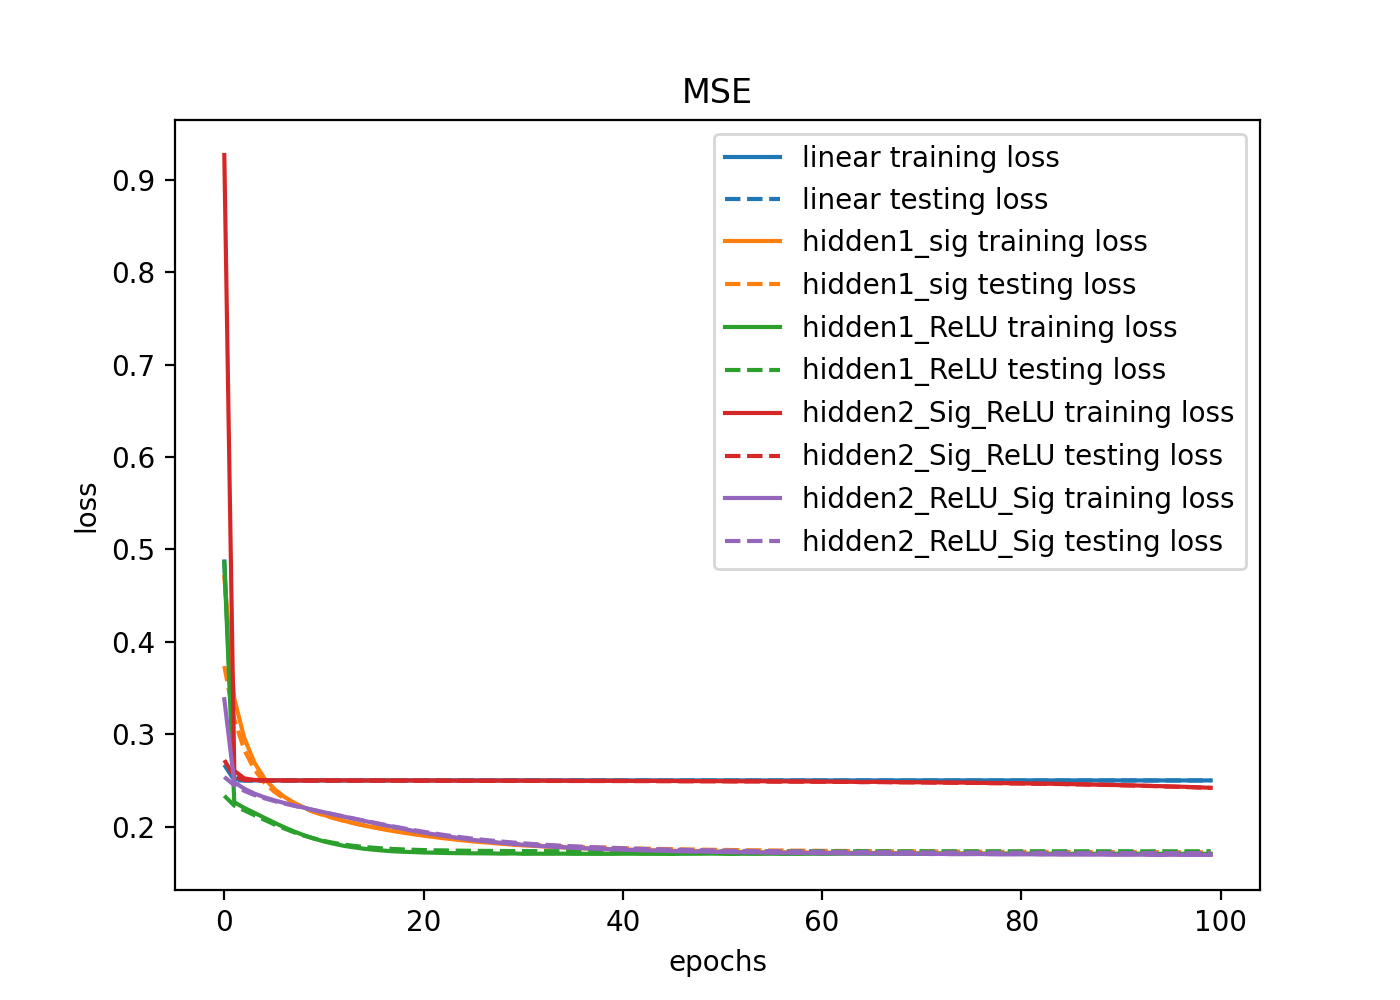
\includegraphics[width=0.4\textwidth]{a4_lossepoch_mse.png}
                \caption{MSE training loss (solid) and test loss (dashed) vs. epochs.}\label{fig:a4_mse}
            \end{figure}
            \begin{figure}[h]
                \centering 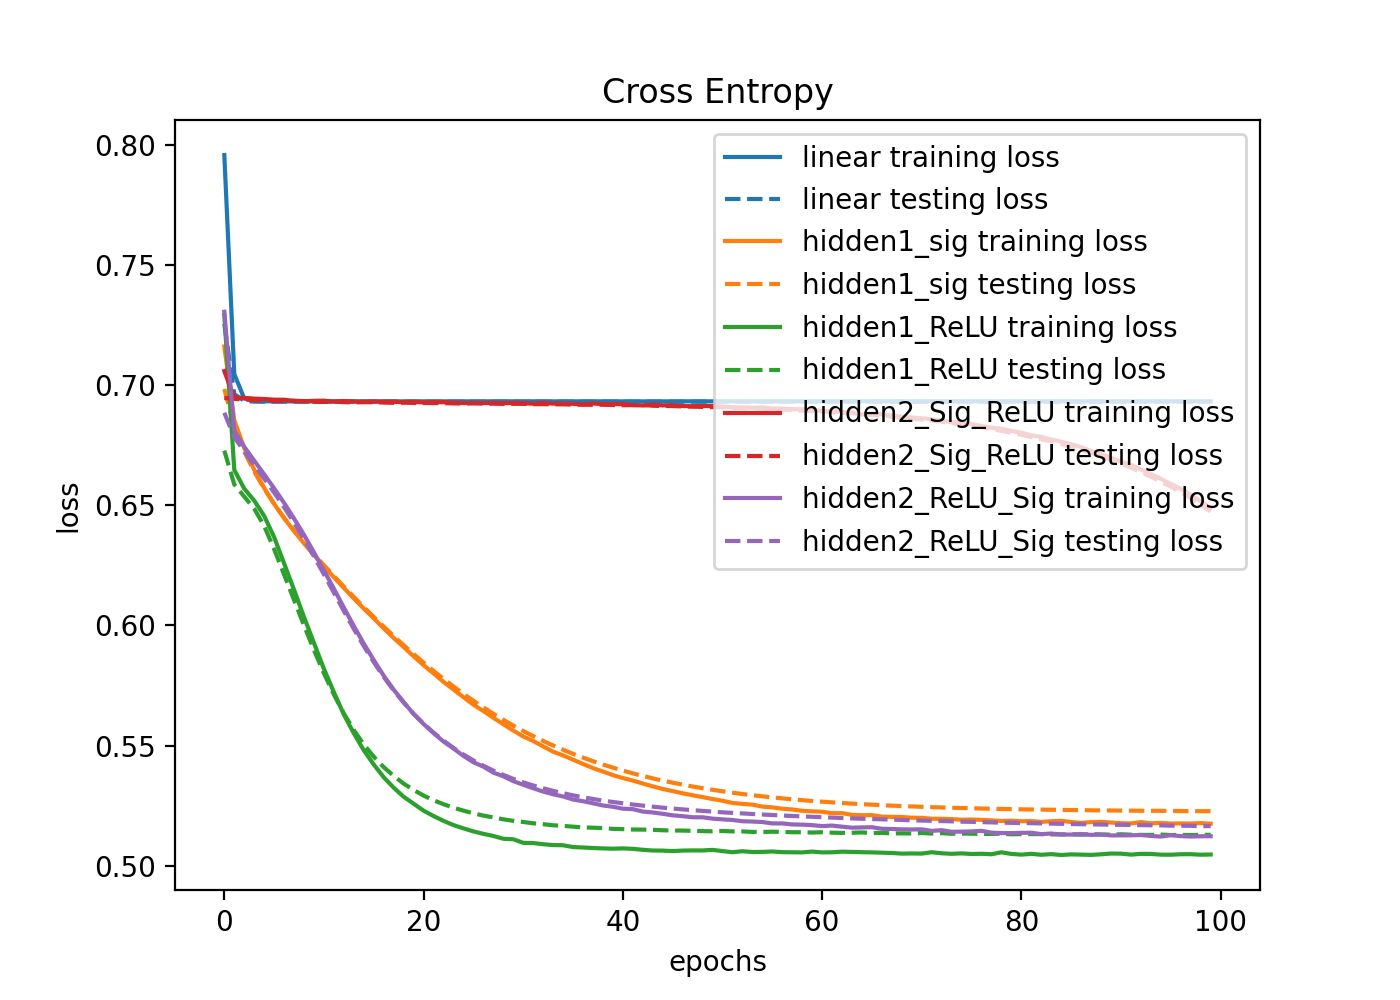
\includegraphics[width=0.4\textwidth]{a4_cross.png}
                \caption{Cross Entropy training loss (solid) and test loss (dashed) vs. epochs.} \label{fig:a4_ce}
            \end{figure}

        Figure \ref{fig:a4_ce} is the plot of loss vs epochs for each neural network defined above for the training (solid) and test (dashed) sets using cross entropy.




        \newpage
        \item \points{5} For each loss function, report the best performing architecture (best performing is defined here as achieving the lowest validation loss at any point during the training), and plot it's guesses on test set. You should use function \texttt{plot\_model\_guesses} from \texttt{train.py} file. Lastly, report accuracy of that model on a test set.

        \textbf{Solution:} The best model according to MSE is ReLU Sigmoid with two hidden layers, while for the CE loss says that ReLU is the best model (one hidden layer). This actually changes when I played with the learning rate (for smaller learning rates $<0.1$, I got ReLU; but for $0.1$, I got ReLU Sigmoid, like the MSE). So there is that small caveat but the loss function for larger learning rates was not pretty - I decided to go with a smaller learning rate since we give it 100 epochs Figure \ref{fig:model_guesses_mse} is the result of \texttt{plot\_model\_guesses} for MSE and Fig. \ref{fig:model_guesses_ce} for cross entropy.
        Either way both CE and MSE tell us that ReLU is the best to use whether after the first hidden layer or alone.

        Accuracy MSE = 0.748
        Accuracy CE = 0.7478

        \begin{figure}[h]
            \centering
            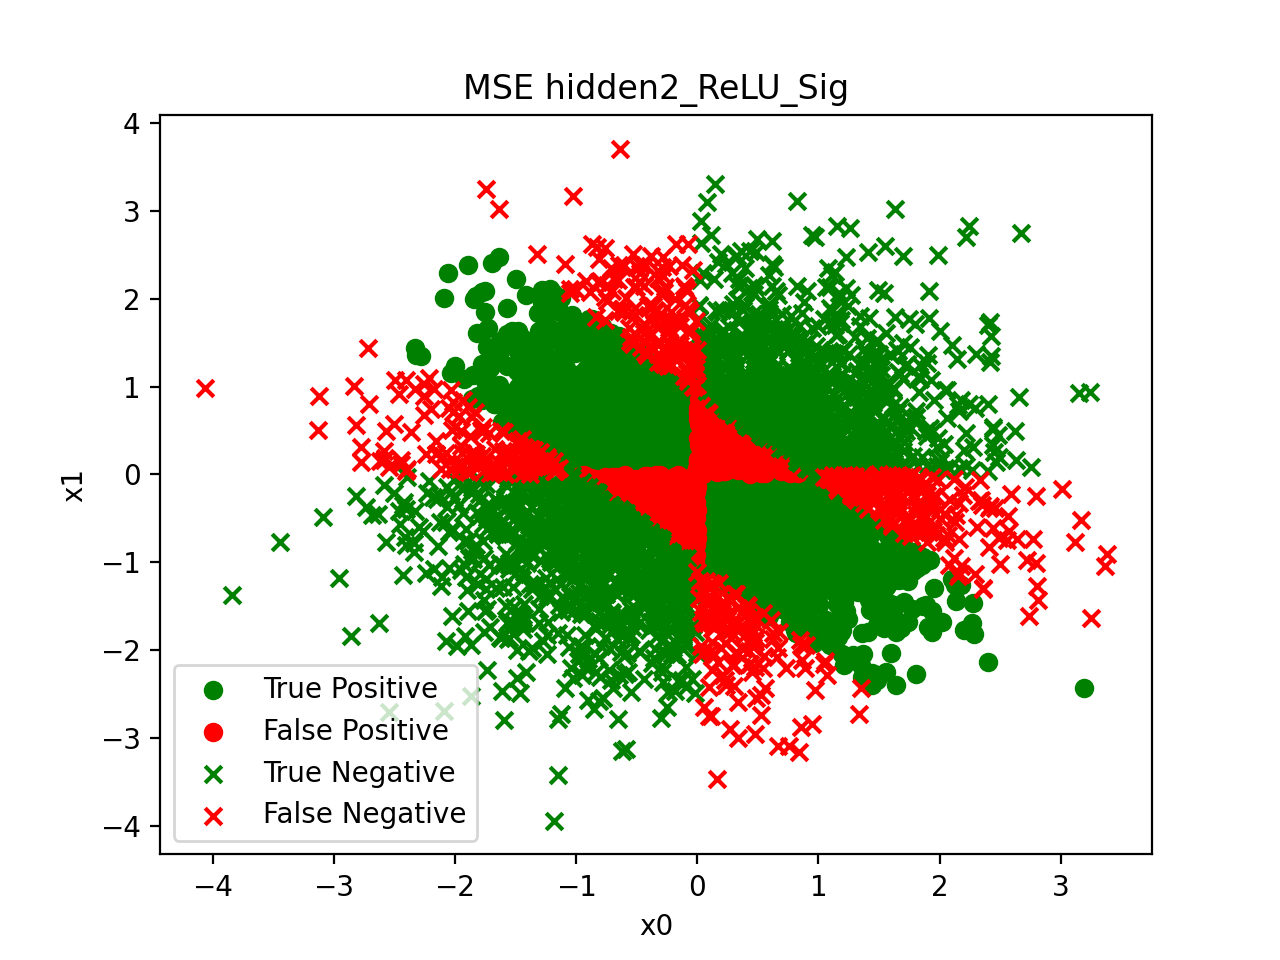
\includegraphics[width=0.5\textwidth]{a4c_mse.png}
            \caption{MSE model guesses}\label{fig:model_guesses_mse}
        \end{figure}

        \begin{figure}[h]
            \centering
            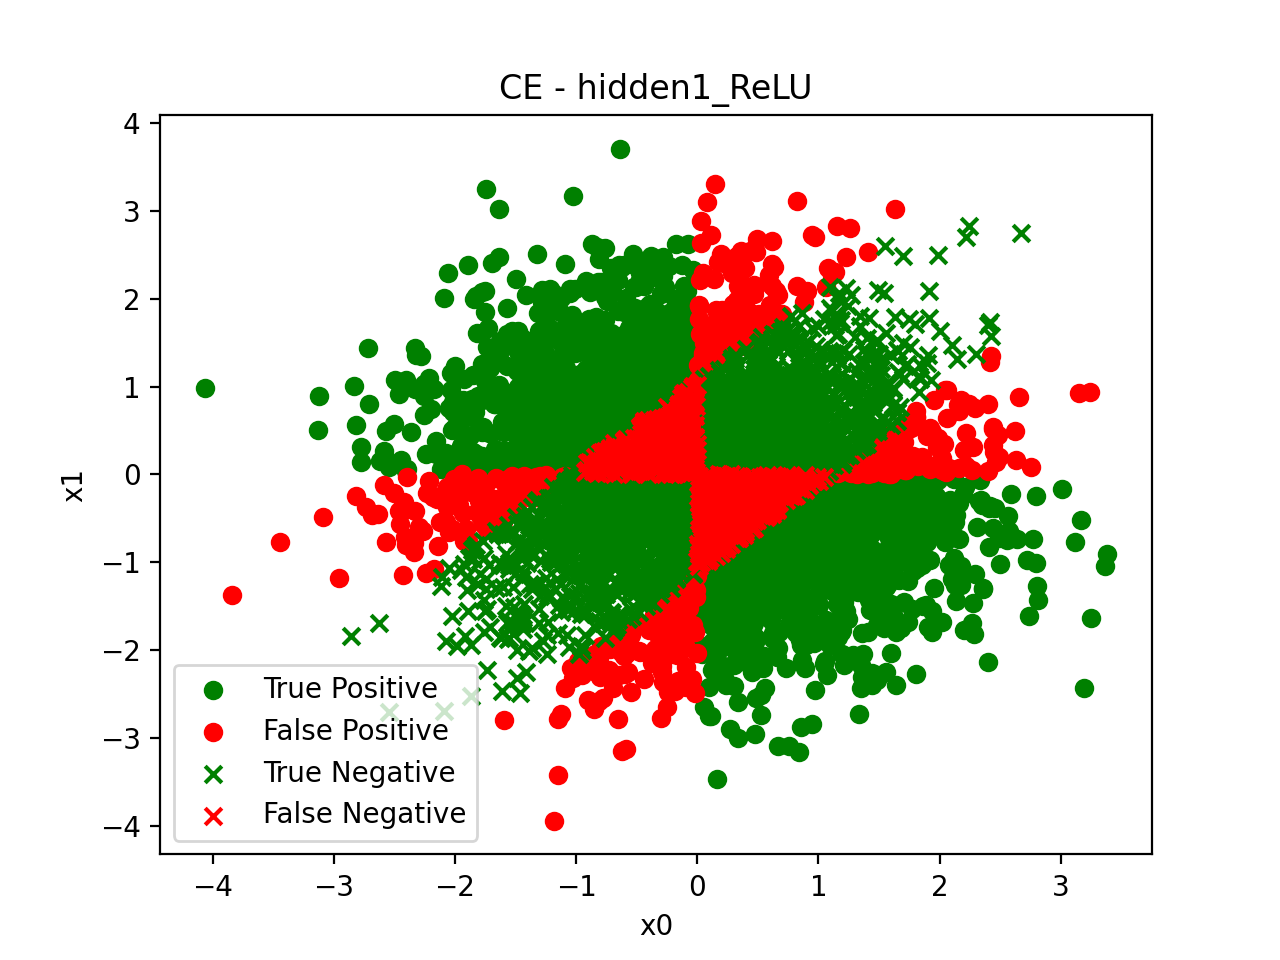
\includegraphics[width=0.5\textwidth]{a4c_cross.png}
            \caption{Cross Entropy model guesses}\label{fig:model_guesses_ce}
        \end{figure}

        \newpage
        \item \points{3} Is there a big gap in performance between between MSE and Cross-Entropy models? If so, explain why it occurred? If not explain why different loss functions achieve similar performance? Answer in 2-4 sentences.
        
        \textbf{Solution:} Yes, there is a gap in the loss functions of MSE and CE. In general we should be using cross entropy for classification problems like this but MSE is fine and still gives us high accuracy (75\%, similar to CE) and acceptable loss function. I played with the learning rate and the gap still existed just at different losses. The difference may arise from the difference in the definition of MSE and CE (and that MSE does better with Gaussian distributions) because the optimizer and the models are otherwise the same (except that cross entropy uses softmax for the models).
    \end{enumerate}
    % \subsubsection*{What to Submit:}
    % \begin{itemize}
    %     \item \textbf{Part b:} 2 plots (one per loss function), with 10 lines each, showing both training and validation loss of each model. Make sure plots are titled, and have proper legends.
    %     \item \textbf{Part c:} Names of best performing models (i.e. descriptions of their architectures), and their accuracy on test set.
    %     \item \textbf{Part c:} 2 scatter plots (one per loss function), with predictions of best performing models on test set.
    %     \item \textbf{Part d:} 2-4 sentence written response to provided questions.
    %     \item \textbf{Code} on Gradescope through coding submission
    % \end{itemize}
\end{aprob}

\newpage
\section*{Neural Networks for MNIST}

    \subsection*{Resources}
        For next question you will use a lot of PyTorch.
        In Section materials (Week 6) there is a notebook that you might find useful.
        Additionally make use of \href{https://pytorch.org/docs/stable/index.html}{PyTorch Documentation}, when needed.

        If you do not have access to GPU, you might find \href{https://colab.research.google.com/}{Google Colaboratory} useful.
        It allows you to use a cloud GPU for free.
        To enable it make sure: "Runtime" -> "Change runtime type" -> "Hardware accelerator" is set to "GPU". When submitting please download and submit a \texttt{.py} version of your notebook.


\begin{aprob}
    \label{code-nn-mnist}
    In previous homeworks, we used ridge regression for training a classifier for the MNIST data set.
    Similarly in previous homework, we used logistic regression to distinguish between the digits 2 and 7.
    
    In this problem, we will use PyTorch to build a simple neural network classifier for MNIST to further improve our accuracy.\\\\
    We will implement two different architectures: a shallow but wide network, and a narrow but deeper network. For both architectures,
    we use $d$ to refer to the number of input features (in MNIST, $d=28^2 = 784$), $h_i$ to refer to the dimension of the $i$-th hidden layer and $k$ for the number of target classes (in MNIST, $k=10$). For the non-linear activation, use ReLU. Recall from lecture that
    \[ \text{ReLU}(x) = \begin{cases} 
          x, & x \geq 0 \\
          0, & x < 0 \ .
       \end{cases}
    \]
    \subsubsection*{Weight Initialization}
    Consider a weight matrix $W \in \mathbb{R}^{n \times m}$ and $b \in \mathbb{R}^n$. Note that here $m$ refers to the input dimension and
    $n$ to the output dimension of the transformation $x \mapsto Wx + b$. Define $\alpha = \frac{1}{\sqrt{m}}$.
    Initialize all your weight matrices and biases according to $\text{Unif}(-\alpha, \alpha)$.
    
    \subsubsection*{Training}
    For this assignment, use the Adam optimizer from \texttt{torch.optim}. Adam is a more advanced form of gradient descent that combines momentum and learning rate scaling. It often converges faster than regular gradient descent in practice. You can use either Gradient Descent or any form of Stochastic Gradient Descent. Note that you are still using Adam, but might pass either the full data, a single datapoint or a batch of data to it. Use cross entropy for the loss function and ReLU for the non-linearity.
    \newpage
    \subsubsection*{Implementing the Neural Networks}
    \begin{enumerate}
        \item \points{10}
        Let $W_0 \in \mathbb{R}^{h \times d}$, $b_0 \in \mathbb{R}^h$, $W_1 \in \mathbb{R}^{k \times h}$, $b_1 \in \mathbb{R}^k$ and $\sigma(z)\colon \mathbb{R} \to \mathbb{R}$
        some non-linear activation function applied element-wise. Given some $x \in \mathbb{R}^{d}$, the forward pass of the wide, shallow network can be formulated as:
        $$\mathcal{F}_1(x) \coloneqq W_1 \sigma(W_0 x + b_0) + b_1$$
        Use $h=64$ for the number of hidden units and choose an appropriate learning rate.
        Train the network until it reaches $99\%$ accuracy on the training data and provide a training plot (loss vs. epoch).
        Finally evaluate the model on the test data and report both the accuracy and the loss.

        \textbf{Solution:} Training plot of loss vs. epoch for F1 model in Figure \ref{fig:lossepoch1}.
        \begin{figure}[h]
            \centering
            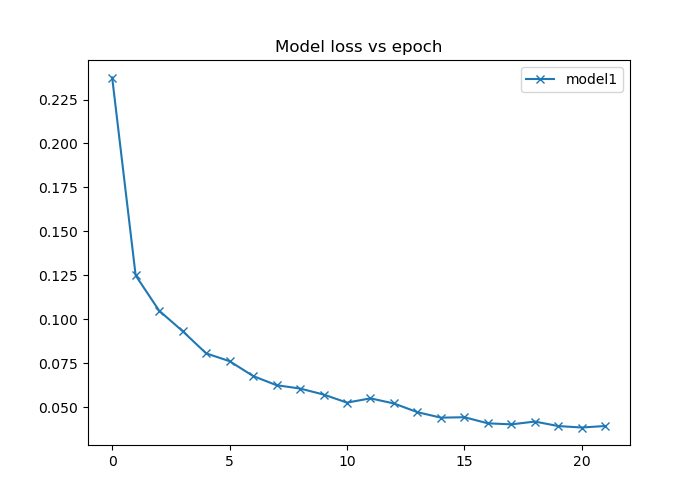
\includegraphics[width=0.5\textwidth]{F1_epochs_loss.png}
            \caption{Loss vs epoch for the training set for F1 model.}
            \label{fig:lossepoch1}
        \end{figure}


        For the test set: \\
        \textbf{F1 model:} Loss = 6.3526e-08, Accuracy = 0.97 \\

        \newpage
        \item \points{10}
        Let $W_0 \in \mathbb{R}^{h_0 \times d}$, $b_0 \in \mathbb{R}^{h_0}$, $W_1 \in \mathbb{R}^{h_1 \times h_0}$, $b_1 \in \mathbb{R}^{h_1}$,
        $W_2 \in \mathbb{R}^{k \times h_1}$, $b_2 \in \mathbb{R}^{k}$ and $\sigma(z) : \mathbb{R} \rightarrow \mathbb{R}$
        some non-linear activation function. Given some $x \in \mathbb{R}^{d}$, the forward pass of the network can be formulated as:
        $$\mathcal{F}_2(x) \coloneqq W_2 \sigma(W_1 \sigma(W_0 x + b_0) + b_1) + b_2$$
        Use $h_0 = h_1 = 32$ and perform the same steps as in part a.

        \textbf{Solution:} Training plot of loss vs. epoch for F2 model in Figure \ref{fig:lossepoch2}.
        \begin{figure}[h]
            \centering
            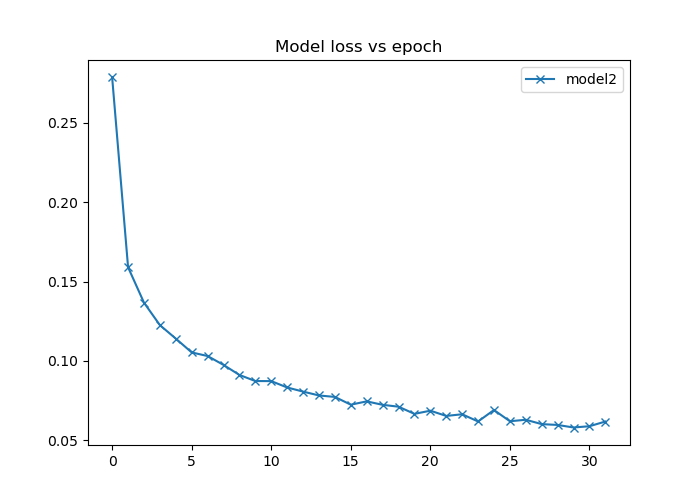
\includegraphics[width=0.5\textwidth]{F2_epochs_loss.png}
            \caption{Loss vs epoch for the training set for F2 model.}
            \label{fig:lossepoch2}
        \end{figure}


        For the test set: \\
        \textbf{F2 model:} Loss = 0.00089, Accuracy = 0.96 \\
        \newpage
        \item \points{5}
        Compute the total number of parameters of each network and report them.
        Then compare the number of parameters as well as the test accuracies the networks achieved. Is one of the approaches (wide, shallow vs. narrow, deeper) better than the other? Give
        an intuition for why or why not.

        \textbf{Solution:}
        Number of parameters: F1 = 50890; F2 = 26506. \\
        Test accuracy: F1 = 0.97; F2 = 0.96 \\

        Wide and shallow is better. I guess maybe the deep but narrow network might be missing out on some semi-significant parameters. Even though it is not as good as the wide and shallo (but still pretty good), it is simpler to understand because it has less variables or parameters to consider. 

    \end{enumerate}

    % \textcolor{red}{\textbf{Using PyTorch:}} For your solution, you may not use any functionality from the \texttt{torch.nn} module except for \texttt{torch.nn.functional.relu},  \texttt{torch.nn.functional.cross\_entropy}, \texttt{torch.nn.parameter.Parameter} and \texttt{torch.nn.Module}. You must implement the networks $\mathcal{F}_1$ and $\mathcal{F}_2$ from scratch. For starter code and a tutorial on PyTorch refer to the sections 6 and 7 material.
    % \subsection*{What to Submit:}
    % \begin{itemize}
    %     \item \textbf{Parts a-b:} Provide a plot of the training loss versus epoch. In addition evaluate the model trained on the test data and report the accuracy and loss.
    %     \item \textbf{Part c:} Report the number of parameters for the network trained in part (a) and for the network trained in part (b).  Provide a comparison of the two networks as described in part in 1-2 sentences.
    %     \item \textbf{Code} on Gradescope through coding submission.
    % \end{itemize}
\end{aprob}

\newpage
\section*{Administrative}
\begin{aprob}
\begin{enumerate}
    \item \points{2} About how many hours did you spend on this homework? There is no right or wrong answer :)
    
    \textbf{24 hours} - three straight days of doing no other work :(, too long - code took forever because I always make a thousand dumb mistakes as well as struggling to figure out what to do... but I really enjoyed A2 and A3.
\end{enumerate}
\end{aprob}



\end{document}